\section{Historique et quelques statistiques sur le Big Data : }
L'expression «Big Data» serait apparue en octobre 1997 selon les archives de la bibliothèque numérique de l'Association for Computing Machinery (ACM)\footnote{\textbf{ACM :} littéralement «association pour les machines de calcul» est une association internationale à but non lucratif, la première à être vouée à l'informatique. Sa mission consiste à développer et soutenir la recherche scientifique et l'innovation informatique.} 
, dans un article scientifique sur les défis technologiques à relever pour visualiser les «grands ensembles de données».

Il apparaît depuis fréquemment dans la presse et dans les revues universitaires, et des programmes de «Data Science» ont vu le jour dans le monde universitaire au cours des six dernières années. Le 29 mars 2012, WHOSTP\footnote{\textbf{WHOSTP: }en français Le Bureau de la politique scientifique et technologique de la Maison Blanche} a annoncé la "Big Data Research and Development Initiative" qui s'appuie sur des initiatives fédérales "allant de l'architecture informatique et des technologies de mise en réseau aux algorithmes, à la gestion des données, à l'intelligence artificielle, apprentissage automatique, développement et déploiement de cyber infrastructures avancées".

Au cours des six dernières années, au moins 17 programmes de science des données ont commencé dans les principales universités de recherche américaines et Internet regorge de publicités pour des livres et des cours de science des données. 

Selon l'étude Data Age 2025, la sphère de données mondiale passera de 33 zettaoctets en 2018 à 175 Zo d'ici 2025. Près de 30\% des données mondiales devront être traitées en temps réel et le stockage réalisé sur le Cloud public représentera 49\% du volume total de données.

Pour ce qui est des statistiques le moins qu'on puisse c'est qu'elles sont impressionnants voici une figure qui permet de représenter la quantité de données générée en 60 secondes d'Internet en 2020 
\textit{(Les données relevées ont été reprises de la compagnie Domo \footnote{\textbf{Domo: } est une société de logiciels cloud, spécialisé dans les outils de business intelligent et la visualisation de données.} qui les a elle-même synthétisées à partir de nombreuses sources hétérogènes)} :

\begin{figure}[h]
	\centering
    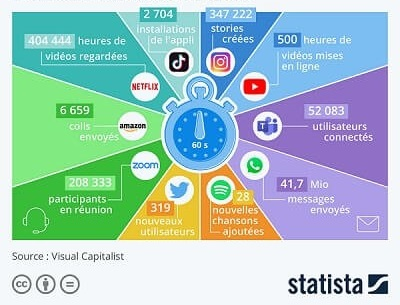
\includegraphics[scale=0.8]{img/part1/1.1}
    \caption{1 minute d'Internet}
\end{figure}

En analysant la \textbf{figure 1.1} on constate l'énorme quantité de données qui circule.  En effet, durant cette minute sur internet alors que les utilisateurs de Facebook publient 147 000 photos, ceux d'Instagram partagent 347 222 stories et Twitter attire 319 nouveaux abonnés. Les plateformes de streaming ne sont pas en reste avec le SVOD Netflix notamment où les utilisateurs visionnent plus de 400 000 heures de vidéo en l'espace de 60 secondes et durant ce même laps de temps, 500 heures de vidéo sont publiées sur Youtube.